\documentclass{article}
\usepackage{listings}
\usepackage[table]{xcolor}
\usepackage{varioref}
\usepackage{float}
\usepackage{graphicx}
\usepackage{geometry} %gives less margins automagically
\begin{document}
\lstset{basicstyle=\ttfamily} % fixed-width listings

\title{KUB manual}
\date{\today}
\author{Tomas H\"ardin}

\maketitle

\newpage

\tableofcontents
\listoffigures
\listoftables

\newpage

\section{Greeting}
Hello world!



Culpa aliquid aperiam consequatur iste aut corrupti. Eos non harum dolor corrupti magnam consequuntur quod. Eos et quam culpa asperiores inventore ad distinctio sunt. Non in alias facilis quam quis vero quod dignissimos. Culpa ipsam velit quia. Ipsa eum enim repudiandae ut sunt doloribus.

Aut assumenda aut asperiores. Rerum ut nihil quisquam et. Quia et tempora vel. Illo excepturi soluta repellendus id debitis. Totam fuga doloribus exercitationem eius.

Et dolores amet id velit. Et ab saepe suscipit temporibus iusto. Odio dicta error voluptas veritatis ab ut aut doloribus. Et facere illo autem ea saepe accusantium eos minus.

Quis quidem porro tempora consequatur. Voluptatibus adipisci quibusdam illo magnam. Ut consequatur quia ipsum. Enim ea tenetur mollitia sed quaerat et neque officiis. Nostrum harum explicabo ut.

Culpa quia voluptas cumque officia. Impedit est ad et assumenda dolorem ex et. Voluptatem atque alias dicta ratione laborum modi rem.

\section{Assembly}


The instrument consists of a stainless steel skeleton into which a number of plates are screwed.
All plates have a printed circuit board (PCB) attached via standoffs or screwed directly to the plate.
The combination of board and plate is called a module.
In this section we assume all PCBs have already been soldered and cleaned.

The following tools and materials are needed:

\begin{itemize}
\item Wire cutters
\item Wire strippers suitable for 0.4 mm and 0.9 mm diameter wire (26 and 20 AWG). Strippers with fixed holes are recommended
\item A small round or semi-round file
\item Torque wrenches capable of 0.3 Nm, 0.8 Nm and 2.0 Nm with the following bits:
\begin{itemize}
\item PH1 Phillips
\item 9IP Torx-Plus or T10 Torx
\item 4.5 mm hex socket
\item 5.5 mm hex socket
\item 7.0 mm hex socket
\end{itemize}
\item Loctite 638
\item Scotch-Weld 2216
\item Soldering station
\item Helping hands
\item 60/40 or 63/37 leaded solder
\item Solder flux
\item White gloves for handling silver
\item Two fine paintbrushes
\item Citadel Chaos Black primer
\item The Army Painter WP1101 Matt Black
\item Electrolube SCP03G Silver Conductive Paint
\item Toothpicks
\item Heat gun
\item 0.62 $mm^2$ / 20 AWG Alpha Wire 5856 WH005 PTFE wire
\item 2.4 mm $\rightarrow$ 1.2 mm Kynar shrink tube
\item Masking tape
\item Maxon EC motor can vice (3D printed)
\end{itemize}

The subsections that follow are ordered in the recommended order of assembly.
The way the pin headers fit into corresponding sockets mean that the power4 module must be mounted first,
then the cpu3 and credits modules can be mounted, and finally the fieldmill9 modules can be mounted.
It's useful to mount the credits module last so that the mating of the fieldmill9 and cpu3 modules can be checked,
and power-on tests performed.

In order to figure out what ID each DS18B20Z 1-wire temperature sensor has
the instrument should be powered on after each module has been installed and
a temperature measurement performed.
The exception to this is when installing power4 and cpu3,
since both are required to get an initial reading and both have a temperature sensor.
Touching the DS18B20Z IC on the power4 board at this phase, thus warming it,
should be enough to distinguish the two at that phase.

Use white gloves when handling any silver parts, to prevent them from being contaminated.
Each aluminium plate requires 16 silver plates M3 screws (?? mm long, Torx T10) to mount it to the skeleton, 96 total.

All M3 screws are torqued to 0.8 Nm and all M2 screws are torqued to 0.3 Nm.

\subsection{power4}

Parts needed:

\begin{itemize}
\item One (1) power4 PCB, soldered and cleaned
\item One (1) silver plated bottom aluminium plate (2mm thick)
\item Two (2) power4 aluminium standoffs
\item Four (4) PEEK washers (top kind)
\item Four (4) PEEK washers (bottom kind)
\item Twentyfour (24) silver plated M3 screws, ?? length inluding head (Torx T10)
\item Four (4) pieces of Alpha Wire 5856 WH005 PTFE wire (TODO: length)
\item 2.4 mm $\rightarrow$ 1.2 mm Kynar shrink tube
\item One (1) DE-9 male connector
\item A set of DE-9 panel mounting screws, washers and nuts
\item Zip ties
\end{itemize}

Solder the four PTFE wires to the DE-9 connector, see figure TODO.
Use Kynar shrink tubing to protect the solder points.

Fasten the DE-9 connector to the aluminium plate (inside or outside??) using the screws, washers and nuts.
Torque to 0.8 Nm.
Screw the standoffs to the plate, 0.8 Nm.

Solder the four PTFE wires to the appropriate places on the power4 board, see figure TODO.
Zip tie the wires together at both ends or in the middle if there isn't enough room.

Place bottom PEEK washers on the standoffs, then the power4 board on the standoffs and finally the top wasters on top.
Screw everything in place using M3 screws, 0.8 Nm.

Screw the finished module to the skeleton using M3 screws, 0.8 Nm.

\subsection{cpu3}

Parts needed:

\begin{itemize}
\item One (1) cpu3 PCB, soldered and cleaned
\item One (1) silver plated cpu3 aluminium plate
\item One (1) cpu3/credits aluminium standoff, short kind
\item One (1) cpu3/credits aluminium standoff, long kind
\item Four (4) PEEK washers (top kind)
\item Four (4) PEEK washers (bottom kind)
\item Twentyfour (24) silver plated M3 screws, ?? length inluding head (Torx T10)
\end{itemize}

Be careful to use the aluminium plate with holes countersunk in the correct direction.
The credits plates are mirror images of the cpu3 plates.

Screw the standoffs to the plate using M3 screws, 0.8 Nm.

Places bottom PEEK washers, board and top PEEK washers on the standoffs.
Screw in place using M3 screws, 0.8 Nm.

Screw the finished module to the skeleton using M3 screws, 0.8 Nm.

Perform a power-on test.
Distinguish the two DS18B20Z temperature sensors now in the instrument by touching one of them, thus warming it.
Write down which ID corresponds to which of the two sensors.

\subsection{fieldmill9}

Parts needed:

\begin{itemize}
\item One (1) fieldmill9 / fieldmill\_top\_plate4 PCB assembly
\item One (1) fieldmill aluminium top plate
\item One (1) fieldmill shutter plate
\item One (1) Maxon 349694 EC motor
\item Stencil with a 15x5 mm hole
\item Two (2) 100 µm stainless steel motor shims
\item One (1) ITR20001/T IR reflex coupler
\item Three (3) M2 screws, 6 mm length including head (Phillips PH1)
\item Four (4) silver plated M3 screws, 10 mm length including head (Torx T10)
\item Sixteen (16) silver plated M3 screws. Same as above??
\item Four (4) M3 washers
\item Four (4) M3 hex nuts
\item One (1) M4 X 8/8 hex screw with 2 mm hole drilled through, preferably silver plated or silver painted if {\it someone} forgot to order silver plated M4 screws
\item One (1) silver plated M4 flange nut
\end{itemize}

Before doing anything else, perform the following electrical tests using a multimeter

\begin{itemize}
\item Check connections to every +2.5V and -2.5V regulator. There's eight ($4 + 4 = 8$) regulators per board
\item Measure resistance from GND to every rail; +3.3V, +24V, +5V, -5V, every +2.5V and every -2.5V. Measure in both directions. Values should all be at least 1 k$\Omega$
\item Measure resistance from either side of R56 to GND. Measure in both directions. Value should be at least 8 k$\Omega$
\item Measure resistance across every NANOSMD PTC. Direction is not important. Values should be no more than 10 $\Omega$. Each board has thirteen (13) PTCs
\end{itemize}

Applying power while these values are out of spec may cause PERMANENT DAMAGE to op-amps, DACs and/or linear regulators.
In the worst case the +-5V regulator (TMR 6-2421WI) may also become damaged.
Once checked and within spec the assembly process may continue:

Cut motor wires to 6-7 mm length.
Strip so that 3 mm of insulation remains, with the wire stripper set to 0.4 mm.
Twist and tin the ends of the wires. See figure \vref{motorwires}.

\begin{figure}
\centering
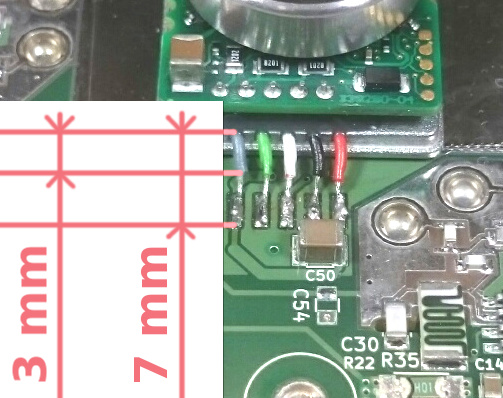
\includegraphics[width=12cm]{3mm7mm}
\caption{Motor wires soldered to their pads. Wire and insulation lengths marked.}
\label{motorwires}
\end{figure}

Put the stencil on the rotor can, tape it down using masking tape and paint the area matt black.
One way to do this is to spray primer into a glass or glazed ceramic cup then dip a fine paintbrush into the primer and paint it onto the can.
DO NOT USE A PLASTIC CUP TO HOLD THE PRIMER - IT WILL MELT.
Wait at least 30 minutes for the primer to dry, then apply the matt black paint on top of it.
The black painted area should cover roughly a 90° arc of the edge of the can.
See figure \vref{reflectometer}.

\begin{figure}
\centering
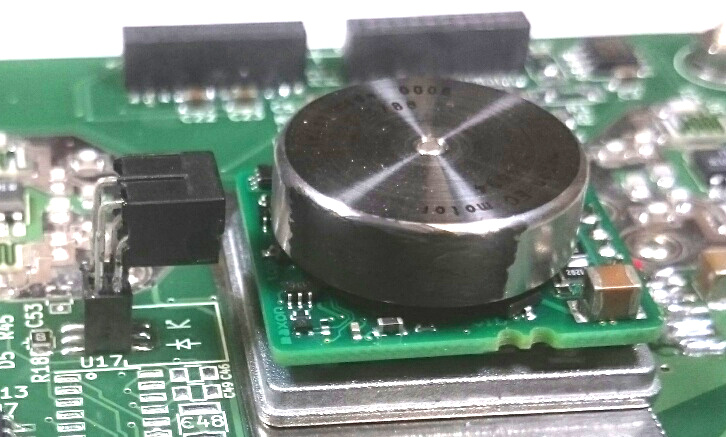
\includegraphics[width=12cm]{reflectometer}
\caption{Reflex coupler and motor can. Black paint also visible on motor can.}
\label{reflectometer}
\end{figure}

Use a small semi-round file to grind away the perforation remains in the middle hole of the PCB,
so that a motor will fit loosely.

Mount the Maxon EC motor in the motor hole with two motor shims inbetween.
The shims should raise the motor enough that a small lip / edge can be felt on the top side of the assembly between the motor housing and the fieldmill\_top\_plate4 PCB.
Solder the five motor wires to the motor wire pads on the PCB.

Bend and cut the IR reflex coupler leads so that the reflex coupler looks directly at the EC motor's rotor can when inserted into its 2x3 socket (IR2 reference on PCB). See figure \vref{reflectometer}.
Bending then trimming all leads to the same length as the shortest lead will accomplish this,
The resulting lead length should be 7 mm from the bottom of the reflex coupler.
Insert the reflex coupler into its socket.
The gap between the top of the 2x3 socket and the bottom of the reflex coupler should be 2 - 3 mm.
Solder the reflex coupler into the socket. Use plenty of flux so the leads and socket are guaranteed to be soldered together.
Some extra solder can be applied to the 2x3 socket pads at this point.
Carefully test that pulling on the reflex coupler doesn't cause it to come out.
Check continuity with a multimeter, and that adjacent pins aren't shorted.

Screw the motor + PCB assembly to the aluminium plate using the M2 screws for the motor and silver plated M3 screws, washers and nuts for the PCB.
First screw in the screws lightly, then tighten using the torque wrench. Use 0.3 Nm for the M2 screws and 0.8 Nm for the M3 nuts.

Use a toothpick to paint the motor bearing with SCP03G silver paint.
Be careful not to get silver paint on the motor axis.
There should be a slight resistance in the bearings which will go away after the first initial minutes of operation.

Use Loctite 638 to glue the M4 screw to the motor axis.
Mount the screw so that the head points downward, toward the instrument,
and so that it is flush with the inner ring of the motor bearing.
When the glue has dried, put the motor can in the specially shaped vice.
Put the shutter plate on the M4 screw and fasten it using the M4 flange nut.
Torque to 2.0 Nm.
Drop some SCP03G silver paint into the top of the screw so that it gets a good electrical connection to the motor shaft.

Screw each module to the skeleton using M3 screws, 0.8 Nm.

Perform a power-on test.
Check that the +5V, -5V and +3.3V rails, and every +2.5V and every -2.5V rail are as expected.
Measure the output of every channel while VGND = 0 V. The average voltage of each output should be within +- 200 mV of VGND.

Take a temperature reading after each fieldmill9 module has been inserted,
and make a note of the new sensor ID each time and what module it corresponds to.

Start the motors and run them for at least five minutes.
Measure the resistance between motor axis and instrument ground.
The resistance should be less than 10 $\Omega$.

\subsection{credits}

\begin{itemize}
\item One (1) credits PCB, soldered and cleaned
\item One (1) silver plated credits aluminium plate
\item One (1) cpu3/credits aluminium standoff, short kind
\item One (1) cpu3/credits aluminium standoff, long kind
\item Four (4) PEEK washers (top kind)
\item Four (4) PEEK washers (bottom kind)
\item Twentyfour (24) silver plated M3 screws, ?? length inluding head (Torx T10)
\end{itemize}

Be careful to use the aluminium plate with holes countersunk in the correct direction.
The credits plates are mirror images of the cpu3 plates.

Screw the standoffs to the plate using M3 screws, 0.8 Nm.

Places bottom PEEK washers, board and top PEEK washers on the standoffs.
Screw in place using M3 screws, 0.8 Nm.

Screw the finished module to the skeleton using M3 screws, 0.8 Nm.

Perform a power-on test and a temperature test.
Take note of the new temperature sensor ID.

\section{Command and response summary}

All commands are human-readable, start with a single ASCII character and are termianted with a line ending.
Comments may be added by inserting a hash sign ('\#').
This causes the rest of the line to be ignored (characters are consumed and discarded until end-of-line).
Mistakes can be corrected with backspace (BS, ASCII code 8) or delete (DEL, ASCII code 127), both of which are treated as a backspace.
Line reading also understands escape (ESC, ASCII code 27), which aborts the current command.

Parameter parsing is handled by sscanf(), which allows for the same command character to take a varying number
of parameters. An example of this is the 'M' command which exists in two-parameter and three-parameter forms:

\begin{lstlisting}
    M0 10       # Set speed of motor 0 to 10
    M10 10 10   # Set speed of all motors to 10
\end{lstlisting}


Line endings can either be carriage return ('{\textbackslash}r', ASCII code 13) or linefeed ('{\textbackslash}n', ASCII code 10), but never both in the same line.
In other words both Unix and Mac line endings are OK, but Windows line endings ("{\textbackslash}r{\textbackslash}n") are not.
This ensures that {\it echo}, {\it minicom} and {\it picocom} work as expected.
Output from the instrument is however terminated by Windows line endings ("{\textbackslash}r{\textbackslash}n"), in order to play nice with {\it minicom} and {\it picocom}.
An ESC ('{\textbackslash}x1B', ASCII code 27) anywhere in a line aborts that command.
The instrument will respond to ESC immediately.
There is no need to terminate ESC with newline.

Output from the instrument is delimited into frames.
A frame start with the string "BEGIN{\textbackslash}r{\textbackslash}n" and ends with the string "END{\textbackslash}r{\textbackslash}n".
Each frame is of a specific type, which is given on the line after BEGIN and preceded by a start (*) and terminated by {\textbackslash}r{\textbackslash}n.
For example, the reply to the "M10 10 10" command example given earlier is of type MTR\_PWM and would therefore be:

\begin{lstlisting}
    BEGIN
    *MTR_PWM
    10 10 10
    END
\end{lstlisting}

Tables \ref{command_table_0} and \ref{command_table} summarize all commands and their parameters.
More detailed descriptions of each command and response are given in the sections that follow.

\definecolor{lgray}{gray}{0.95}
\definecolor{dgray}{gray}{0.90}

\begin{table}[H]
\begin{centering}
\rowcolors{1}{lgray}{dgray}
\begin{tabular}{|p{1.0cm}|p{7.8cm}|p{2.0cm}|}
\hline
{\bf Char} & {\bf Description}    & {\bf Response}\\ \hline
v & Measure system voltages       & VOLTAGES      \\ \hline
V & Enable 24V and +-5V           & VOLTAGES      \\ \hline
B & Disable 24V and +-5V          & VOLTAGES      \\ \hline
m & Read motor PWMs               & MTR\_PWM      \\ \hline
K & Set motor PWMs to 50\%        & MTR\_PWM      \\ \hline
r & Measure motor speeds in RPM   & MTR\_SPD      \\ \hline
1 & List 1-wire device ROMs       & ONEWIRE       \\ \hline
! & Search for 1-wire devices     & ONEWIRE       \\ \hline
t & Measure temperatures          & TEMPS         \\ \hline
c & Read clock in cycles          & CLOCK         \\ \hline
U & UNLOCK all ADS131A04          & ADC\_REGS     \\ \hline
q & Read ADS131A04 registers      & ADC\_REGS     \\ \hline
S & Reboot                        & {\emph None}  \\ \hline
? & Print help                    & INFO          \\ \hline
{\textbackslash}x1B (ESC)  &   Stop measurement, abort current recvline().
Can occur anywhere in a line, does not have to be terminated with newline. & ESC \\ \hline
\end{tabular}
\caption{Command table, parameterless commands}
\label{command_table_0}
\end{centering}
\end{table}

\begin{table}[H]
\begin{centering}
\rowcolors{1}{lgray}{dgray}
\begin{tabular}{|p{0.8cm}|p{2.6cm}|p{4.9cm}|p{2.0cm}|}
\hline
{\bf Char} & {\bf Parameter syntax} & {\bf Description} & {\bf Response} \\ \hline
M & id pwm              & Set motor PWM                       & MTR\_PWM      \\ \hline
M & pwm0 pwm1 pwm2      & Set all motor PWMs                  & MTR\_PWM      \\ \hline
Q & id addr val [...]   & Set ADS131A04 registers             & ADC\_REGS     \\ \hline
  &                     & Read CPU regs (\$0000 - \$00FF)     &               \\ \hline
  &                     & Write CPU regs (\$0000 - \$00FF)    &               \\ \hline
  &                     & Read RAM (\$0100 - \$FFFF)          &               \\ \hline
  &                     & Write RAM (\$0100 - \$FFFF)         &               \\ \hline
  &                     & Read EEPROM (\$000 - \$FFF)         &               \\ \hline
  &                     & Write EEPROM (\$000 - \$FFF)        &               \\ \hline
  &                     & Read ROM (\$00000 - \$1FFFF)        &               \\ \hline
  &                     & Read fuses                          &               \\ \hline
C & cycles              & Set clock in cycles                 & CLOCK         \\ \hline
w & cycles              & Wait given number of cycles         & INFO          \\ \hline
  &                     & Configure measurement (block size + gap) &               \\ \hline
  &                     & Read measurement configuration      &               \\ \hline
  &                     & Start measurement                   &               \\ \hline
\end{tabular}
\caption{Command table, commands with parameters}
\label{command_table}
\end{centering}
\end{table}

\section{Responses}

Responses given before commands since many commands share response format.

\subsection{INFO}

Informative text.
Display contents in text window or terminal.
Should be displayed with normal colors.
Example:

\begin{lstlisting}
    BEGIN
    *INFO
    Starting temperature conversion...
    END
\end{lstlisting}


\subsection{WARNING}

Warning.
Should be displayed with a yellowish or maybe orange color.

\begin{lstlisting}
    BEGIN
    *WARNING
    Instrument issues no warnings currently,
    but may in the future.
    END
\end{lstlisting}


\subsection{ERROR}

Some kind of error.
Should be displayed with a reddish color.

\begin{lstlisting}
    BEGIN
    *ERROR
    One or more of PWMS 1111, 2222, and 3333
    is greater than MOTOR_TOP = 1023
    END
\end{lstlisting}


\subsection{VOLTAGES}

TODO

\subsection{MTR\_PWM}

PWM value for each of the three motors, as integers between 0 - 1023.
These correspond roughly to 0 - 6000 RPM, but not exactly.
For more information see EC20 datasheet.
Example response after issuing a "K" command:

\begin{lstlisting}
    BEGIN
    *MTR_PWM
    511 511 511
    END
\end{lstlisting}

\subsection{MTR\_SPD}

Motor speeds in RPM, and the number of tachometer impulses detected.
For a sensible output at least two tachs must have been seen for each motor.
Exact format isn't finalized, so display output as if it were INFO for now.

\begin{lstlisting}
    BEGIN
    *MTR_SPD
    Motor 0: 0 tachs (0 RPM)
    Motor 1: 1 tachs (0 RPM)
    Motor 2: 2 tachs (1234 RPM)
    END
\end{lstlisting}

\subsection{ONEWIRE}

1-Wire devices.
One line per device containing a 64-bit hexadecimal ROM string (16 characters).

\begin{lstlisting}
    BEGIN
    *ONEWIRE
    28d09948090000ec
    286a1a690900005e
    28ad7548090000c5
    END
\end{lstlisting}

\subsection{TEMPS}

Temperature readings.
One line per DS18B20Z device with 64-bit hexadecimal ROM and decimal temperature values in degrees Celsius.
Range is -40..+125 with a resolution of 1/16 degrees Celsius.

\begin{lstlisting}
    BEGIN
    *TEMPS
    28d09948090000ec 24.12
    286a1a690900005e 24.62
    28ad7548090000c5 -18.56
    END
\end{lstlisting}

\subsection{CLOCK}

Current time in CPU cycles as a 64-bit decimal value.
May roll over in theory, but it would take 79,000 years unless the user
specifically set the clock to something close to the maximum value (18446744073709551615).

\begin{lstlisting}
    BEGIN
    *CLOCK
    3702994144
    END
\end{lstlisting}

\subsection{SAMPLES}

Sample data.
This response is binary.
It is possible, but very unlikely, that the binary data contains the string "END{\textbackslash}r{\textbackslash}n".
To avoid trouble it is best to compute the exact number of bytes in the sample data by following listing \vref{sample_packet_s}.

\begin{lstlisting}
    BEGIN
    *SAMPLES
    [sample_packet_s]
    END
\end{lstlisting}

\subsection{ADC\_REGS}

The contents of all registers in all ADCs.
Three lines, each beginning with the integer ID of the ADC.
After this there are twenty-one (21) hexadecimal values corresponding to registers 00h - 14h.
See ADS131A04 datasheet for more information.

This example has one fieldmill installed in position 1.
Therefore only the middle line (ID=1) has valid data:

\begin{lstlisting}
    BEGIN
    *ADC_REGS
    0 ff ff ff ff ff ff ff ff ff ff ff ff ff ff ff ff ff ff ff ff ff
    1 04 03 00 00 00 00 00 01 00 00 00 60 3c 08 86 00 00 00 00 00 00
    2 ff ff ff ff ff ff ff ff ff ff ff ff ff ff ff ff ff ff ff ff ff
    END
\end{lstlisting}

The first two registers (ID\_MSB and ID\_LSB) can be used to detect that an ADC is working,
since they are read-only and of known value.
All our chips have ID\_MSB = 04h (for ADS131A{\emph 04}) and ID\_LSB = 03h (revision 3).

\section{Commands}

\subsection{Reboot ('S')}

Takes no parameters and no prisoners.
Hangs the user program, inducing the WDT to cause a software reset.
After the reset the CPU enters the bootloader.
This allows a serial programmer to keep sending 'S' to get the device into a known state,
since the AVR109 bootloader merely responds to 'S' with 'AVRBOOT'.
If no programming is performed then the user program is re-entered after the bootloader wait time has elapsed (typically three seconds).

\begin{lstlisting}
    S
    S
    AVRBOOT[three second delay]BEGIN
    *INFO
    Hello, Earth! 👽
    END
\end{lstlisting}


\subsection{Set motor PWMs ('M')}

Set one or more OCR1x.
PWM values must be between 0 - 1023.

\subsubsection{Two parameter form (id pwm)}

\subsubsection{Three parameter form (pwm0 pwm1 pwm2)}

\subsection{Set ADS131A04 registers ('Q')}

The 'Q' command can set one or more registers in one or more of the ADCs.
It is given as a series of lines and terminated by a blank line.
Each line must contain three values: an integer specifying the ADC ID,
a hexadecimal value specifying the register address and a hexadecimal value specifying the value.
In C formatting parlance it should be "\%i \%x \%x".
The first line should also begin with 'Q'.
There can be any number of lines.

The following example sets COMP\_TH = 111b and enables fixed word size (6 device words per frame regardless of ADC\_ENA):

\begin{lstlisting}
    Q1 0B 67
    1 0C 3E

    BEGIN
    *ADC_REGS
    0 ff ff ff ff ff ff ff ff ff ff ff ff ff ff ff ff ff ff ff ff ff
    1 04 03 00 00 00 00 00 01 00 00 00 67 3e 08 86 00 00 00 00 00 00
    2 ff ff ff ff ff ff ff ff ff ff ff ff ff ff ff ff ff ff ff ff ff
    END
\end{lstlisting}


\section{Listing}
\label{sample_packet_s}

\lstinputlisting{../app/sample_packet_s.h}



\end{document}
